\subsection{Comparison with Independent Measurements from the Turf-House Monitoring Project}\label{sec:keldur-comparison}

\draftchange{The Keldur measurements in the preceding subsections were compared with a distant weather station, which does not measure the conditions inside the turf. This subsection therefore compares the developed sensor nodes with a second, independent set of in-situ measurements recorded at Keldur during the same period by a separate monitoring project.\footnote{\draftchange{These data were provided by the Department of Civil and Environmental Engineering through the project \textit{Monitoring and Simulation of Hygrothermal and Structural Behaviour of Turf Houses: Towards Preservation and Performance Optimization}.}} The comparison shows whether the developed nodes behave similarly to an independent sensor set. It is not a calibration or an accuracy test, because no sensors were placed at the same location.}

\subparagraph{The two sensor sets}

\draftchange{The project data come from four buried soil sensors, which report soil temperature and dielectric permittivity (a quantity that increases with soil moisture), and from two air sensors, which report temperature and relative humidity. The soil sensors were described as similar in type to the reference instrument used for the calibration in Section~\ref{sec:soil-calibration}; the exact model is not stated in the received file. Table~\ref{tab:cmp-layout} lists the positions, taken from the sensor-placement diagram supplied with the data. The depths in the diagram, given in centimetres, were converted to millimetres.}

\begin{table}[htbp]
\centering
\caption{\draftchange{Sensor positions of the developed nodes and of the project sensors. Depths are measured from the turf surface.}}
\label{tab:cmp-layout}
\small
\begin{tabular}{l l c l}
\hline
Source & Sensor & Depth (mm) & Position \\
\hline
Developed & Node 1 & 80 & Separate roof \\
Developed & Node 3 & 60 & Separate roof \\
Developed & Node 5 & 65 & Separate roof \\
Developed & Node 7 & 85 & Separate roof \\
Project & \#93 & 20 & Upper position, near surface \\
Project & \#94 & 105 & Upper position, bottom of turf layer \\
Project & \#95 & 15 & Lower position, near surface \\
Project & \#96 & 240 & Lower position, bottom of turf layer \\
Project & Inside air sensor & -- & Inside, on top of the wall \\
Project & Outside air sensor & -- & Outside, at the gable window \\
\hline
\end{tabular}
\end{table}

\draftchange{The two deployments differ in an important way. All four project soil sensors are on one side of a single roof, whereas the developed nodes are beneath four separate roofs (Figure~\ref{fig:results-deployment-map}). The exact roof of the project sensors relative to the developed nodes is not marked in the received file. The comparison therefore addresses general behaviour, timing, and order of magnitude, not sensor-by-sensor equivalence.}

\draftchange{Three measurements are compared: soil temperature (all four nodes against all four project soil sensors), air temperature and relative humidity (all four nodes against the project outside air sensor), and soil moisture (Nodes 1, 3, and 7 against the four project soil sensors). The comparison covers the deployment period of the developed nodes for which project data were provided, from 18 October 2025 (the day after the nodes were buried) to 27 January 2026. Both datasets are in UTC and were averaged to hourly and then daily values. For each sensor pair, only the days on which both sensors reported were used. Placeholder entries of the developed nodes (Section~\ref{sec:keldur-individual}) and individual readings of exactly zero were treated as missing. Two measures are used throughout. The correlation coefficient $r$ describes whether two sensors rise and fall together: 1 means they move together perfectly and 0 means they are unrelated. The difference is the developed node minus the project sensor, so a negative value means the node was colder or drier.}

\subparagraph{Soil temperature}

\draftchange{Figure~\ref{fig:cmp-soil-daily} shows the daily mean soil temperature of both sensor sets. They follow the same sequence of events: cooling during the first two weeks after burial, warm periods in the first half of November, a stable low-temperature plateau from mid-November to mid-December (near 0~°C for all sensors except \#96, which stayed at about 2~°C), a warm event at the end of December, and cooling in January for the sensors that were still reporting. The developed nodes were buried beneath four separate roofs, yet their daily means follow this sequence together.}

\begin{figure}[htbp]
\centering
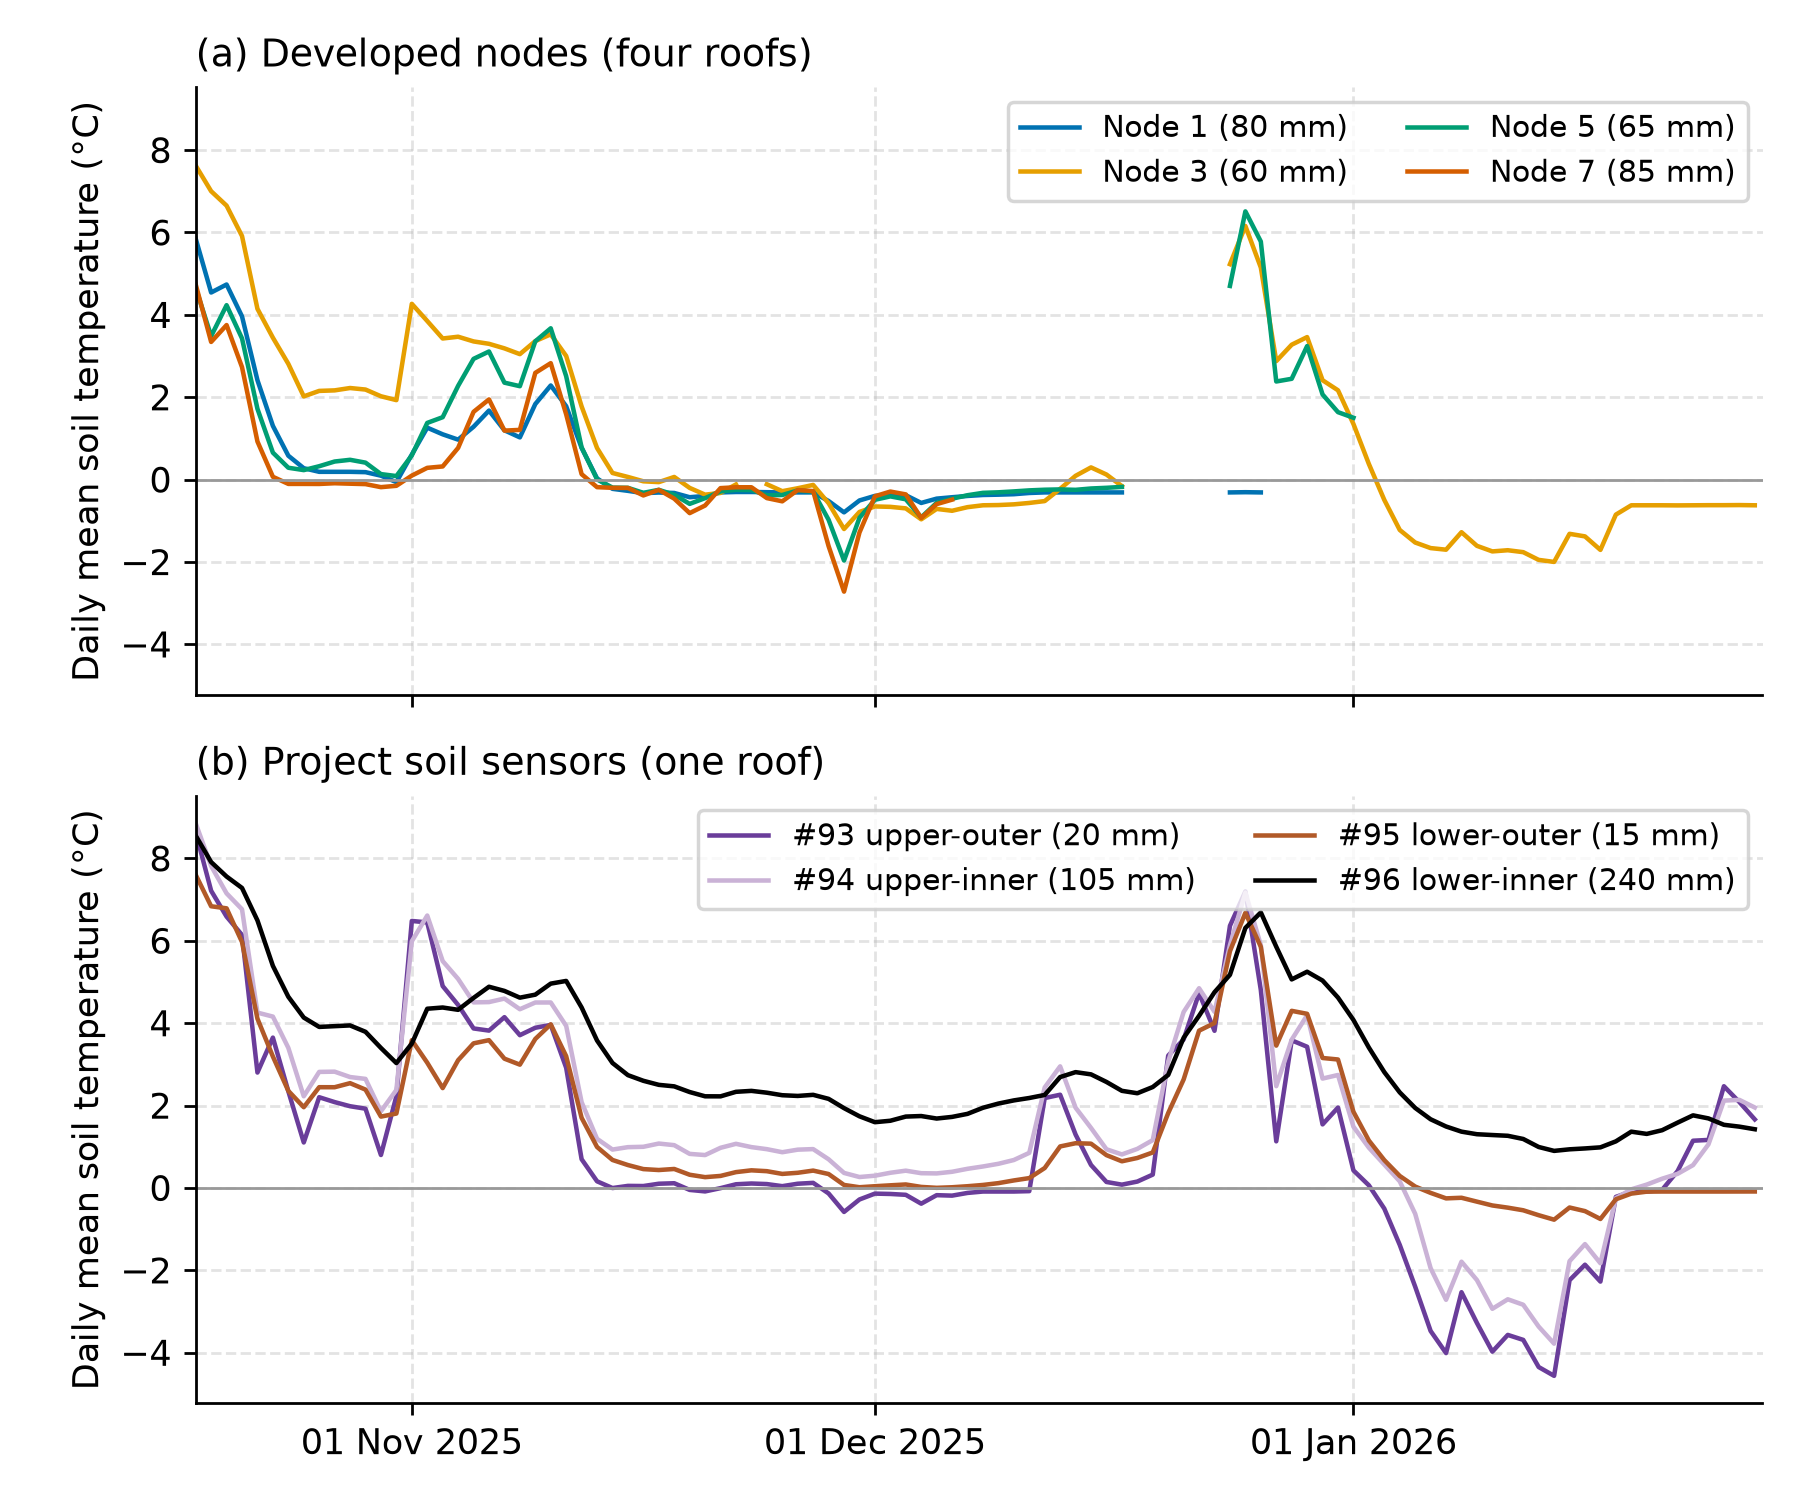
\includegraphics[width=\textwidth,height=0.6\textheight,keepaspectratio]{figs/keldur-compare-soil_temp_daily.png}
\caption{\draftchange{Daily mean soil temperature measured by (a) the four developed nodes and (b) the four project soil sensors.}}
\label{fig:cmp-soil-daily}
\end{figure}

\draftchange{Table~\ref{tab:cmp-soil} and Figure~\ref{fig:cmp-soil-corr} summarise the agreement. Every developed node correlated strongly with every project sensor ($r$ from 0.75 to 0.98), and Node 3 had the strongest agreement ($r \geq 0.91$ for all four project sensors). The developed nodes were on average colder than the project sensors, by 0.16~°C to 3.33~°C. The smallest differences were obtained for Node 3 against the near-surface sensors \#93 and \#95 (0.16~°C and 0.56~°C), and the largest against the deepest and warmest project sensor \#96. For context, the mean soil temperatures of the four project sensors over the whole window already differ by about 2~°C among themselves (1.1~°C to 3.1~°C), so differences of this order between positions are not unusual at this site. The data do not identify whether the remaining offsets are caused by roof location, turf thickness, burial depth, or sensor differences.}

\begin{figure}[htbp]
\centering
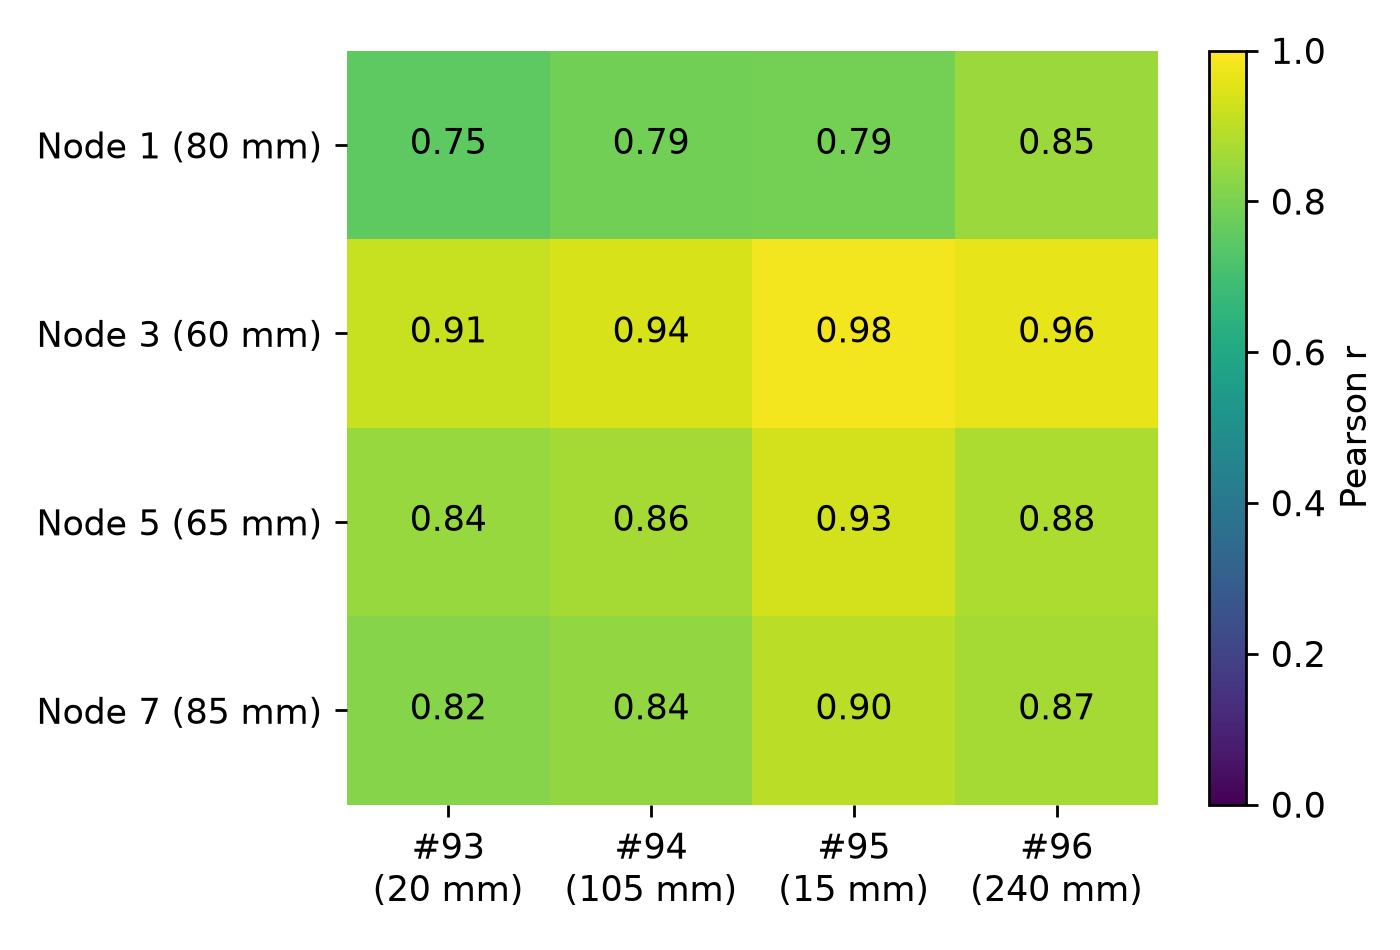
\includegraphics[width=0.75\textwidth,keepaspectratio]{figs/keldur-compare-soil_temp_corr.png}
\caption{\draftchange{Correlation coefficient $r$ between the daily mean soil temperature of each developed node and each project soil sensor. The number of days compared is 64 (Node 1), 95 (Node 3), 70 (Node 5), and 50 (Node 7).}}
\label{fig:cmp-soil-corr}
\end{figure}

\begin{table}[htbp]
\centering
\caption{\draftchange{Difference in daily mean soil temperature between each developed node and the four project soil sensors (\#93--\#96), and the share of hours in which the node reading was within 1~°C of the range spanned by the four project sensors. The difference is the developed node minus the project sensor.}}
\label{tab:cmp-soil}
\small
\setlength{\tabcolsep}{4pt}
\begin{tabular}{l c c c}
\hline
Node & Days compared & Difference (°C) & Hours within 1~°C (\%) \\
\hline
1 & 64 & $-1.48$ to $-3.11$ & 61.5 \\
3 & 95 & $-0.16$ to $-2.20$ & 97.7 \\
5 & 70 & $-1.02$ to $-2.75$ & 75.6 \\
7 & 50 & $-1.64$ to $-3.33$ & 54.0 \\
\hline
\end{tabular}
\end{table}

\subparagraph{Air temperature and relative humidity}

\draftchange{The project outside sensor is the closest counterpart to an ambient air measurement. The inside sensor is in the space on top of the wall and varies much less, so it is not used here. Figure~\ref{fig:cmp-air-rh} compares the daily means of the project outside sensor with all four nodes. Nodes 5 and 7 had exposed atmospheric sensors (solid lines), whereas Nodes 1 and 3 had them inside the enclosure (dashed lines). The enclosed sensors were not expected to represent ambient conditions and are shown for completeness.}

\begin{figure}[htbp]
\centering
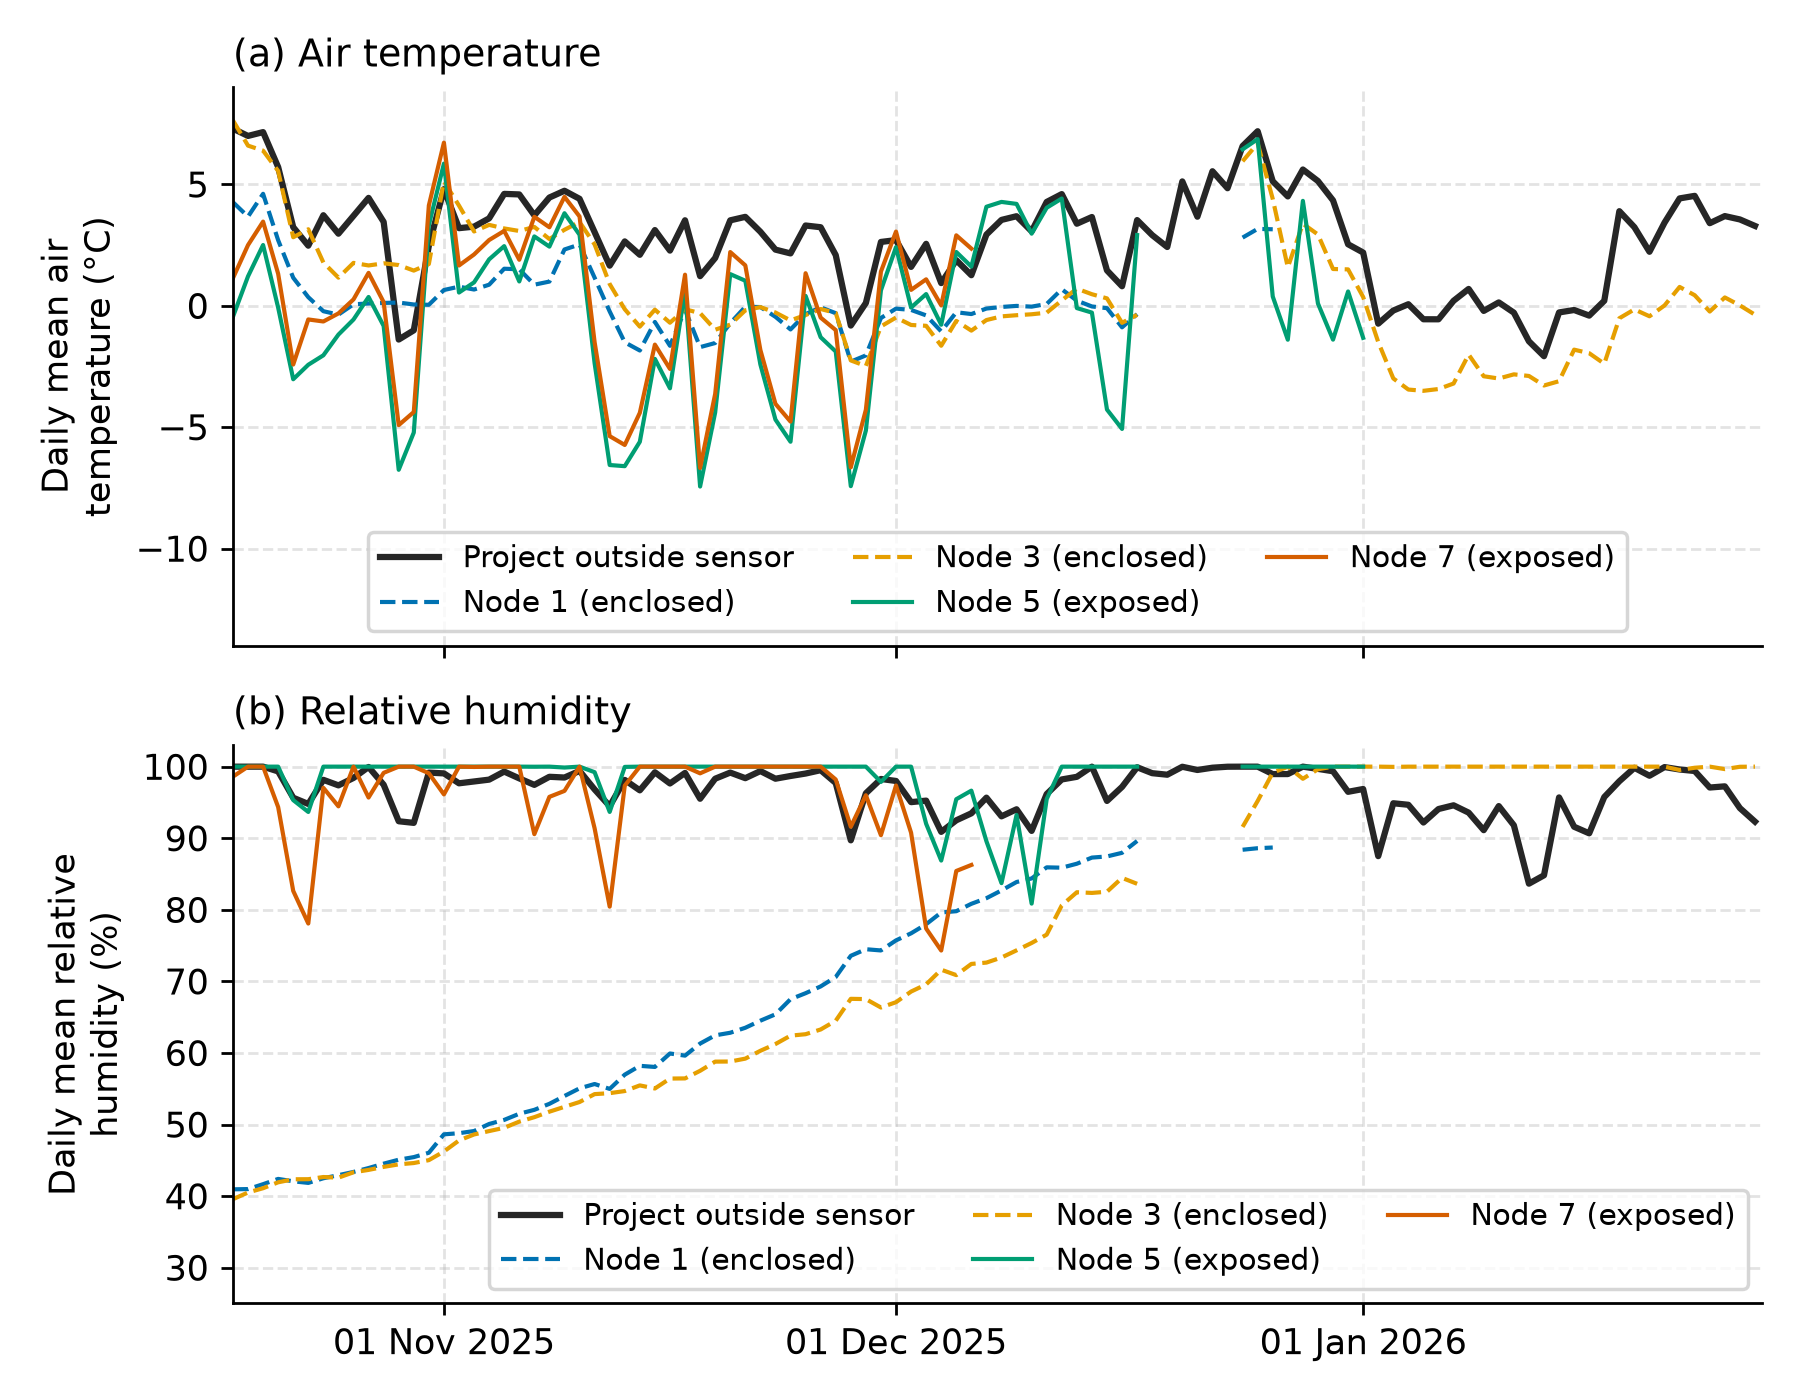
\includegraphics[width=\textwidth,height=0.55\textheight,keepaspectratio]{figs/keldur-compare-air_rh_simple.png}
\caption{\draftchange{Daily mean (a) air temperature and (b) relative humidity of the four developed nodes and of the project outside sensor. Dashed lines are the nodes with enclosed atmospheric sensors (Nodes 1 and 3) and solid lines are the nodes with exposed sensors (Nodes 5 and 7).}}
\label{fig:cmp-air-rh}
\end{figure}

\draftchange{All four nodes followed the day-to-day air-temperature changes of the project outside sensor ($r$ from 0.64 to 0.81, Table~\ref{tab:cmp-air}), but they were colder by 2.2~°C to 3.5~°C on average. The exposed sensors showed larger daily swings (median daily range of 6.65~°C and 7.86~°C for Nodes 5 and 7) than the enclosed sensors (0.76~°C and 1.15~°C) and the project outside sensor (2.14~°C). This agrees with the observation in Section~\ref{sec:keldur-deployment-results} that the enclosed sensors respond more slowly to ambient changes. Because the nodes are on different roofs and the project sensor is at the gable window, the differences in level and daily range cannot be attributed to the sensors alone.}

\draftchange{For relative humidity, the exposed sensors of Nodes 5 and 7 agreed well with the project outside sensor. Their daily means differed on average by only $+1.1$ and $-1.8$ percentage points, and both the nodes and the project sensor spent most hours at or above 95\% relative humidity (89\% and 71\% of the hours for Nodes 5 and 7, against 76\% for the project outside sensor). The enclosed sensors of Nodes 1 and 3 behaved differently. They started near 40\% and rose gradually towards the humidity level recorded by the project sensors, so they did not represent ambient humidity during most of the period. Node 3 then remained near 100\% from late December to the end of the window (daily means of 99.5\% to 100\% from 4 to 27 January), while the project outside sensor recorded daily means between 83.7\% and 99.9\%. The project outside sensor also recorded 99\% or above during 32\% of the hours in January, so near-saturated conditions do occur at the site. However, the cause of the gradual rise of the enclosed sensors is not established, and the readings of Node 3 should still be treated with the caution stated in Section~\ref{sec:keldur-humidity}. These results support the earlier observation that exposed sensors are preferable for monitoring ambient humidity.}

\begin{table}[htbp]
\centering
\caption{\draftchange{Agreement of the developed nodes with the project outside air sensor, calculated from daily means over the days on which both reported. The difference is the developed node minus the project sensor.}}
\label{tab:cmp-air}
\small
\setlength{\tabcolsep}{4pt}
\begin{tabular}{l l c c c c c}
\hline
 & & \multicolumn{2}{c}{Air temperature} & \multicolumn{2}{c}{Relative humidity} & \\
Node & Sensor & $r$ & Difference (°C) & $r$ & Difference (\%) & Days \\
\hline
1 & Enclosed & 0.80 & $-2.88$ & $-0.22$ & $-33.5$ & 64 \\
3 & Enclosed & 0.81 & $-2.19$ & $-0.31$ & $-22.9$ & 96 \\
5 & Exposed & 0.66 & $-3.49$ & 0.62 & $+1.1$ & 70 \\
7 & Exposed & 0.64 & $-3.05$ & 0.60 & $-1.8$ & 50 \\
\hline
\end{tabular}
\end{table}

\subparagraph{Soil moisture trend}

\draftchange{The soil moisture of the two sensor sets cannot be compared directly. The project sensors report dielectric permittivity $\varepsilon$, whereas the developed nodes report raw ADC values. The laboratory calibration in Section~\ref{sec:soil-calibration} links ADC values to permittivity through five points (Table~\ref{tab:final-calibration-results}) that cover ADC values from 197 to 485. Most Keldur ADC readings are above this range (daily medians of about 530 to 580 for Nodes 1, 3, and 7), so the laboratory points cannot be applied to them directly. Node 5 was excluded because its ADC value was constant at 768 for 47.5\% of the hours.}

\draftchange{The laboratory points show a sensitivity of about 0.068 permittivity units per ADC count. In the field, a linear regression of the daily project permittivity on the daily node ADC gave between 0.054 and 0.107 units per count (depending on the node and on the project sensor \#93, \#94, or \#95). The sensitivity of the nodes in the field is therefore similar to the laboratory sensitivity, and the main difference is a large shift of the ADC level. A constant ADC offset was fitted for each node so that the permittivity obtained from the laboratory points falls inside the range spanned by the four project sensors. The offset was fitted on the first half of each node's days and tested on the second half. ADC values that fell outside the laboratory range after the shift were treated as invalid and counted as not matching.}

\draftchange{The fitted offsets were $-254$, $-341$, and $-332$ ADC counts for Nodes 1, 3, and 7 (Figure~\ref{fig:cmp-moisture}). In the fit period, 78\%, 94\%, and 92\% of the days were inside the project range, which is expected because the offset was fitted to these days. In the test period, which gives the real check, 53\%, 75\%, and 88\% of the days were inside the range, and the correlation of the shifted node values with the mean of the project sensors was 0.86, 0.76, and 0.55. Nodes 1 and 3 were often at the lower edge of the project range or just below it during the test period. The shifted values follow the main features of the project data, including the decrease in mid-November, the low values around the beginning of December, and the increase in late December. Independent of the offset, the day-to-day changes of the node ADC values and of the project permittivity had a positive Spearman rank correlation for all combinations of Nodes 1, 3, and 7 with the four project sensors (0.51 to 0.78).}

\draftchange{This result must be interpreted with care. The project range is wide (median width of about 14 permittivity units, for a mean level of about 16), so being inside it is a lenient criterion. The fitted offsets are also large compared with the 288-count laboratory range, and they differ between nodes, so they cannot be treated as a simple calibration offset of the electronics. Possible causes include the soil, the contact between the sensor and the soil, and differences between sensors, but the data do not identify which one applies. The offsets were obtained from the project data, so the comparison shows that the nodes can reproduce the project data after a fitted shift, but it does not establish the absolute accuracy of the nodes. Part of the agreement may also come from a shared response to temperature and freezing, which affects both permittivity and capacitive readings.}

\draftchange{The fitted offsets suggest a recommendation for future deployments. The offsets differed between nodes, which may reflect differences between individual devices as well as differences in soil and installation conditions at each roof. To obtain the best absolute soil-moisture results, it is recommended that each node is characterised in ADC counts before deployment, preferably in soil from the intended site, and that the nodes are installed carefully, with good contact between the sensor and the surrounding soil, so that installation-related errors are avoided. The soil-moisture readings can also be used to follow relative changes over time.}

\begin{figure}[htbp]
\centering
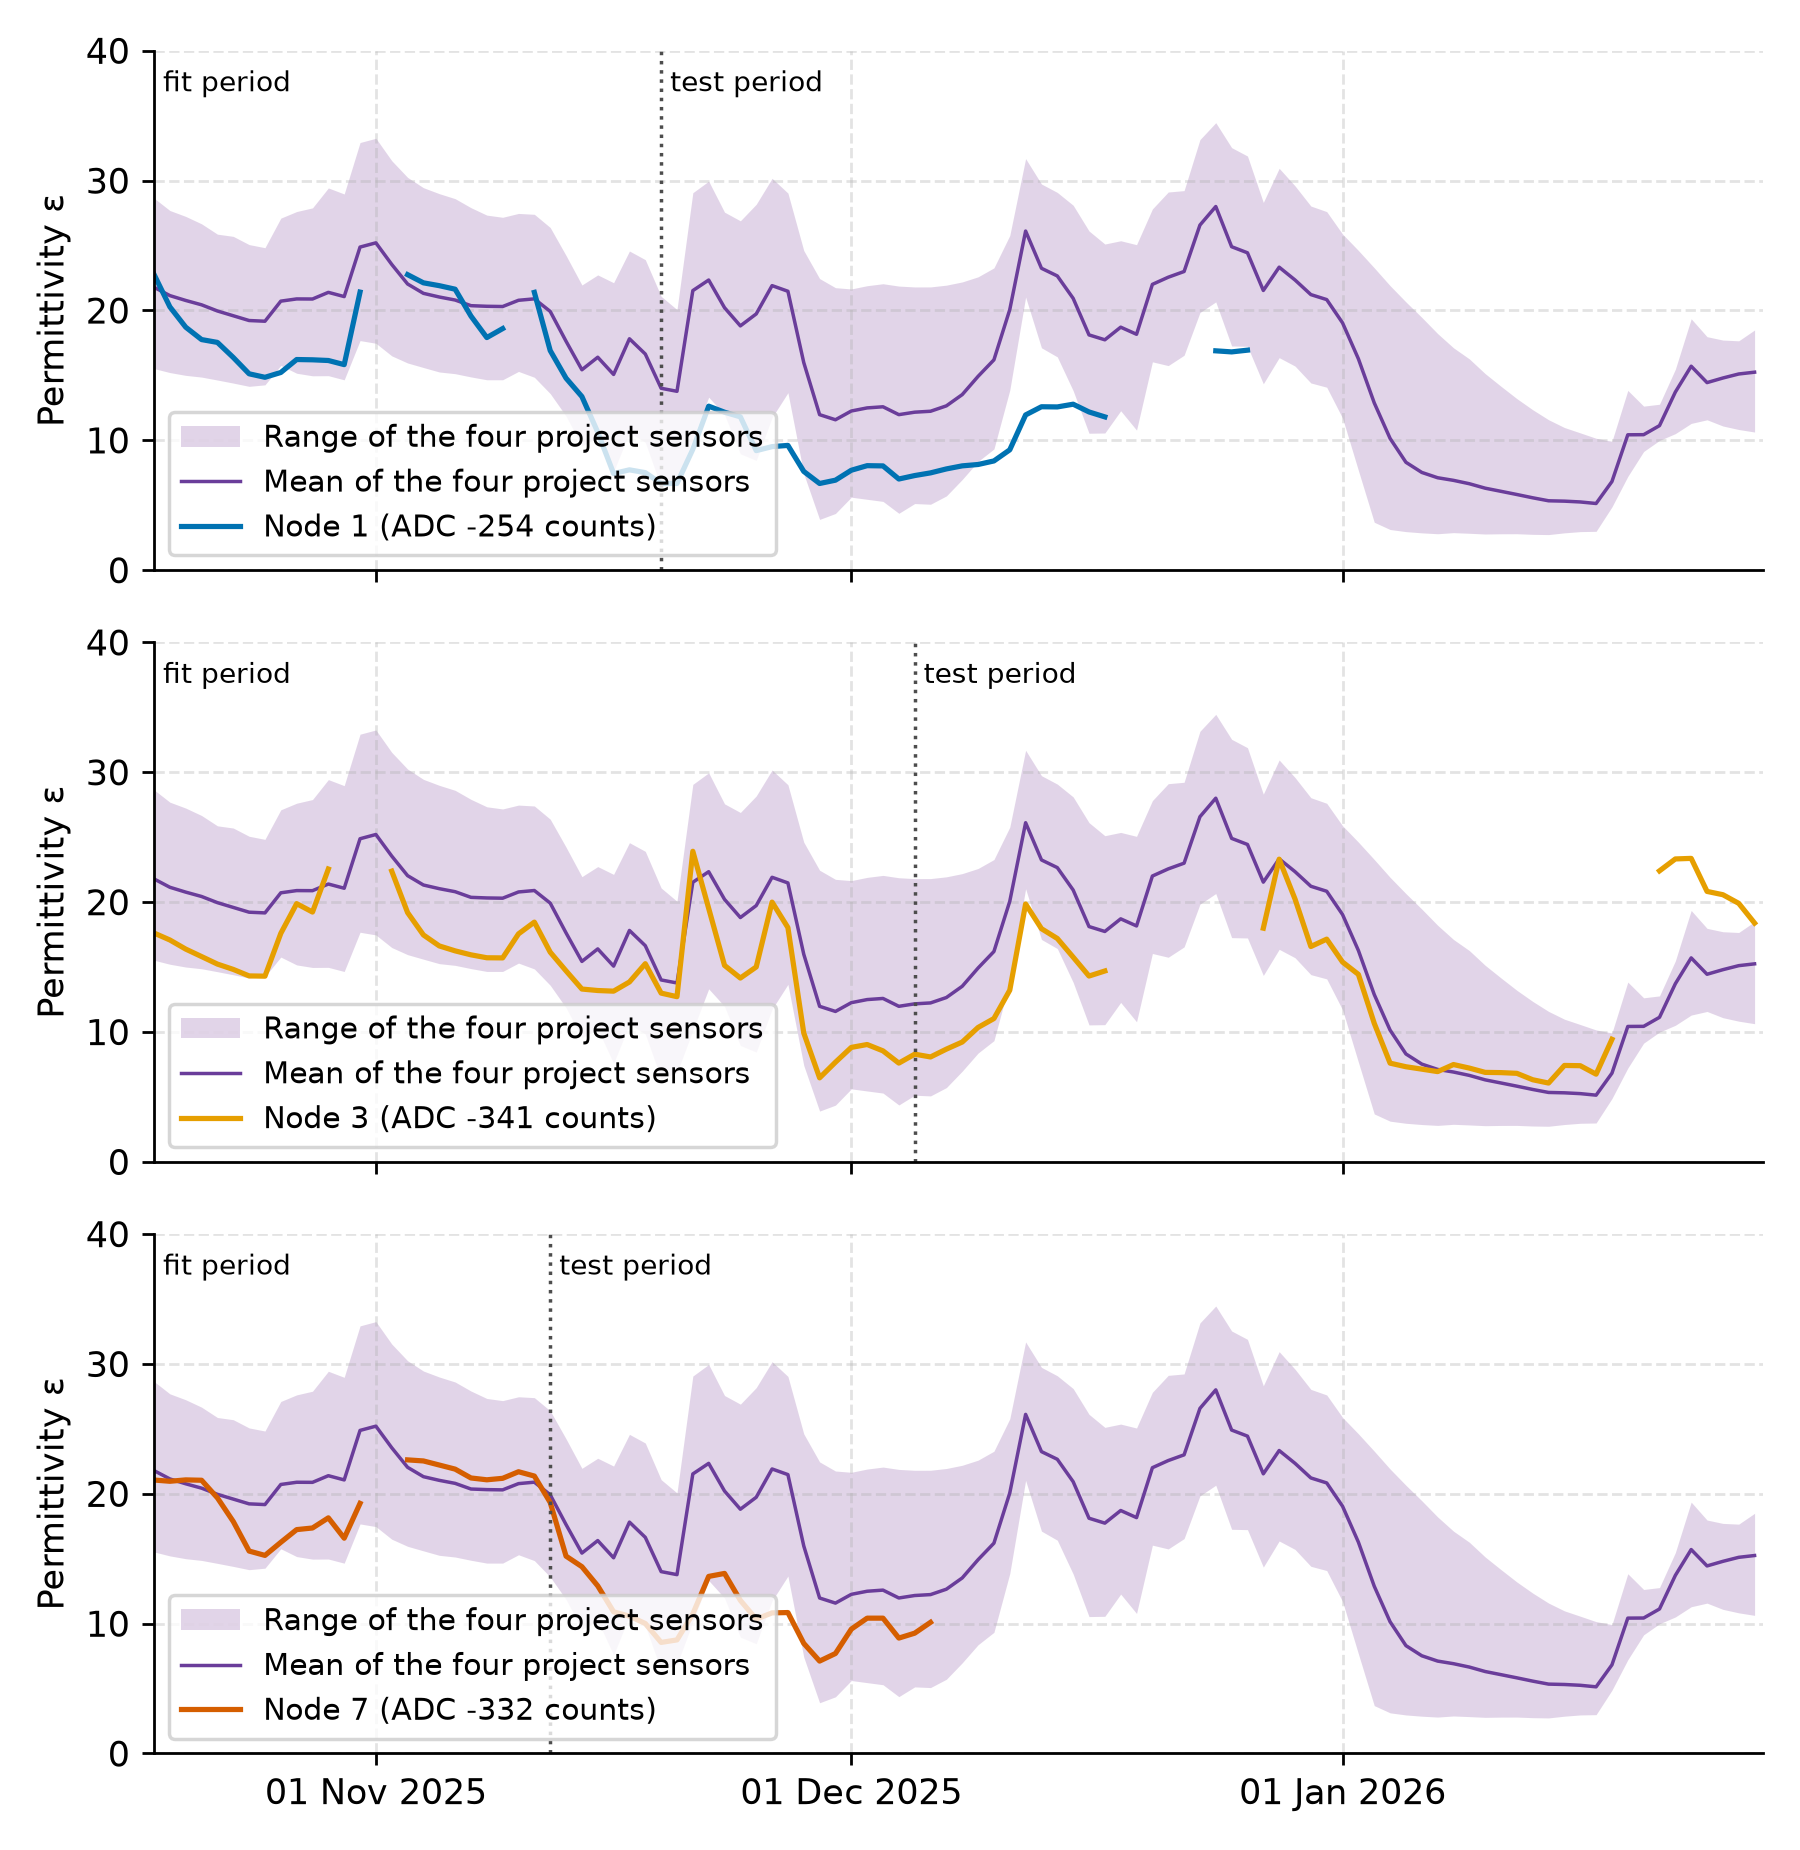
\includegraphics[width=\textwidth,height=0.7\textheight,keepaspectratio]{figs/keldur-compare-moisture_offset.png}
\caption{\draftchange{Permittivity obtained from the ADC values of Nodes 1, 3, and 7 after applying a fitted ADC offset, compared with the range and the mean of the four project soil sensors. The offset was fitted on the days before the dotted line and tested on the days after it. Gaps are days on which the shifted ADC value was outside the laboratory calibration range.}}
\label{fig:cmp-moisture}
\end{figure}

\subparagraph{Summary of the comparison}

\draftchange{The comparison with the independent project measurements gives the following results. The soil temperatures recorded by the developed nodes follow the same temporal pattern as the project sensors, with correlations of 0.75 to 0.98. The exposed humidity sensors of Nodes 5 and 7 agreed with the project outside sensor within 2 percentage points on average, and all four nodes followed the day-to-day air-temperature changes of the project outside sensor. The relative changes in soil moisture of the nodes were positively correlated with the changes in permittivity recorded by the project sensors, and after a fitted ADC offset the permittivity obtained from the nodes followed the main features of the project data.}

\draftchange{The comparison also has limits. The developed nodes were generally colder than the project sensors, the enclosed humidity sensors did not represent ambient humidity, and the deepest project sensor did not follow the same moisture pattern. The project sensors are on one roof and the developed nodes are on four, no sensors were co-located, and the soil-moisture comparison depends on an offset that was fitted to the project data, and node-specific characterisation and careful installation are recommended for future deployments. The results therefore show that the developed system recorded consistent environmental behaviour relative to an independent dataset, but they do not establish the absolute accuracy of the nodes.}
